% Options for packages loaded elsewhere
\PassOptionsToPackage{unicode}{hyperref}
\PassOptionsToPackage{hyphens}{url}
%
\documentclass[
]{article}
\usepackage{amsmath,amssymb}
\usepackage{lmodern}
\usepackage{iftex}
\ifPDFTeX
  \usepackage[T1]{fontenc}
  \usepackage[utf8]{inputenc}
  \usepackage{textcomp} % provide euro and other symbols
\else % if luatex or xetex
  \usepackage{unicode-math}
  \defaultfontfeatures{Scale=MatchLowercase}
  \defaultfontfeatures[\rmfamily]{Ligatures=TeX,Scale=1}
\fi
% Use upquote if available, for straight quotes in verbatim environments
\IfFileExists{upquote.sty}{\usepackage{upquote}}{}
\IfFileExists{microtype.sty}{% use microtype if available
  \usepackage[]{microtype}
  \UseMicrotypeSet[protrusion]{basicmath} % disable protrusion for tt fonts
}{}
\makeatletter
\@ifundefined{KOMAClassName}{% if non-KOMA class
  \IfFileExists{parskip.sty}{%
    \usepackage{parskip}
  }{% else
    \setlength{\parindent}{0pt}
    \setlength{\parskip}{6pt plus 2pt minus 1pt}}
}{% if KOMA class
  \KOMAoptions{parskip=half}}
\makeatother
\usepackage{xcolor}
\IfFileExists{xurl.sty}{\usepackage{xurl}}{} % add URL line breaks if available
\IfFileExists{bookmark.sty}{\usepackage{bookmark}}{\usepackage{hyperref}}
\hypersetup{
  hidelinks,
  pdfcreator={LaTeX via pandoc}}
\urlstyle{same} % disable monospaced font for URLs
\usepackage{graphicx}
\makeatletter
\def\maxwidth{\ifdim\Gin@nat@width>\linewidth\linewidth\else\Gin@nat@width\fi}
\def\maxheight{\ifdim\Gin@nat@height>\textheight\textheight\else\Gin@nat@height\fi}
\makeatother
% Scale images if necessary, so that they will not overflow the page
% margins by default, and it is still possible to overwrite the defaults
% using explicit options in \includegraphics[width, height, ...]{}
\setkeys{Gin}{width=\maxwidth,height=\maxheight,keepaspectratio}
% Set default figure placement to htbp
\makeatletter
\def\fps@figure{htbp}
\makeatother
\setlength{\emergencystretch}{3em} % prevent overfull lines
\providecommand{\tightlist}{%
  \setlength{\itemsep}{0pt}\setlength{\parskip}{0pt}}
\setcounter{secnumdepth}{5}
\ifLuaTeX
  \usepackage{selnolig}  % disable illegal ligatures
\fi

\author{}
\date{}

\begin{document}

\title{MLT Week-7}
\author{Sherry Thomas \\ 21f3001449}

\maketitle
\tableofcontents

\begin{abstract}
This week examines the primary methods of binary classification, namely linear classifiers, K-nearest neighbor (K-NN) algorithm, and decision trees. The advantages and disadvantages of each approach are comprehensively discussed, alongside their efficient implementation.
\end{abstract}

\hypertarget{introduction-to-binary-classification}{%
\section{Introduction to Binary
Classification}\label{introduction-to-binary-classification}}

Binary classification is a machine learning task where the goal is to
classify objects into one of two categories. It is a fundamental problem
in various fields, including computer vision, natural language
processing, and bioinformatics.

Given a dataset \(\{x_1, \ldots, x_n\}\) where \(x_i \in \mathbb{R}^d\),
let \(\{y_1, \ldots, y_n\}\) be the labels, where \(y_i \in \{0, 1\}\).
The goal is given by \(h: \mathbb{R}^d \rightarrow \{0, 1\}\).

The loss for this function is given by, \[
loss(h)=\frac{1}{n}\sum ^n _{i=1}\mathbb{1}\left ( h(x_i) \ne y_i \right )
\] Let \(\mathcal{H}_{\text{linear}}\) represent the solution space for
the mapping in the linear space. \[
\mathcal{H}_{\text{linear}}=\Biggr \lbrace{h_w: \mathbb{R}^d \rightarrow \{1, 0\} \hspace{0.5em} s.t. \hspace{0.5em} h_w(x)=sign(w^Tx) \hspace{0.5em} \forall w \in \mathbb{R}^d } \Biggr \rbrace
\] Therefore, the objective function is given by, \[
\min _{h \in \mathcal{H}_{\text{linear}}} \sum _{i=1} ^n \mathbb{1}\left ( h(x_i) \ne y_i \right )
\] This objective function presents an NP-Hard Problem, indicating the
challenge in arriving at optimal and sufficient parameters. Therefore,
improved implementations are necessary to address this complexity and
achieve satisfactory results.

\hypertarget{linear-classifier}{%
\section{Linear Classifier}\label{linear-classifier}}

Can we use linear regression to solve this classification problem?

The proposed algorithm would be as follows: \[
\{(x_1, y_1), \ldots, (x_n,y_n)\} \xrightarrow[Regression]{Linear} w \in \mathbb{R}^d\rightarrow h_w: \mathbb{R}^d \rightarrow \{1, 0\}
\] But this poses an issue in classification. Look at the diagram below:

\begin{figure}
\centering
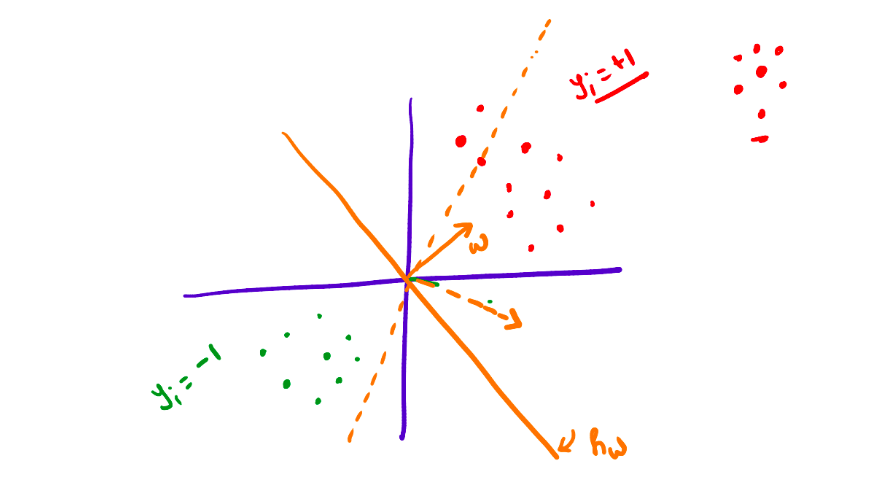
\includegraphics{../images/lin_class.png}
\caption{Linear classification and the problem due to outliers}
\end{figure}

Upon a detailed examination of the above diagram, it is evident that
classification based on Linear Regression not only partitions the two
categories of data based on their respective sides but also their
positions. Consequently, this approach may cause the classification
boundary to shift w.r.t. the outliers in the dataset. Therefore, this
approach is not feasible.

\hypertarget{k-nearest-neighbours-algorithm}{%
\section{K-Nearest Neighbours
Algorithm}\label{k-nearest-neighbours-algorithm}}

The K-Nearest Neighbor (K-NN) algorithm is a popular non-parametric
method used for classification and regression tasks in machine learning.
It operates by identifying the K-nearest data points to the target
object, classifying or regressing the target object based on the
majority of its nearest neighbors.

The algorithm is as follows:

\begin{itemize}
\tightlist
\item
  Given \(x_{test}\) find the \(k\)-closest points in the training set -
  \(\{x_1^*, x_2^*, \ldots, x_k^*\}\).
\item
  Predict \(y_{test} = \text{majority}(y_1^*, y_2^*, \ldots, y_k^*)\)
\end{itemize}

Look at the following diagrams to the see the effect of the value of
\(k\) on the classification:

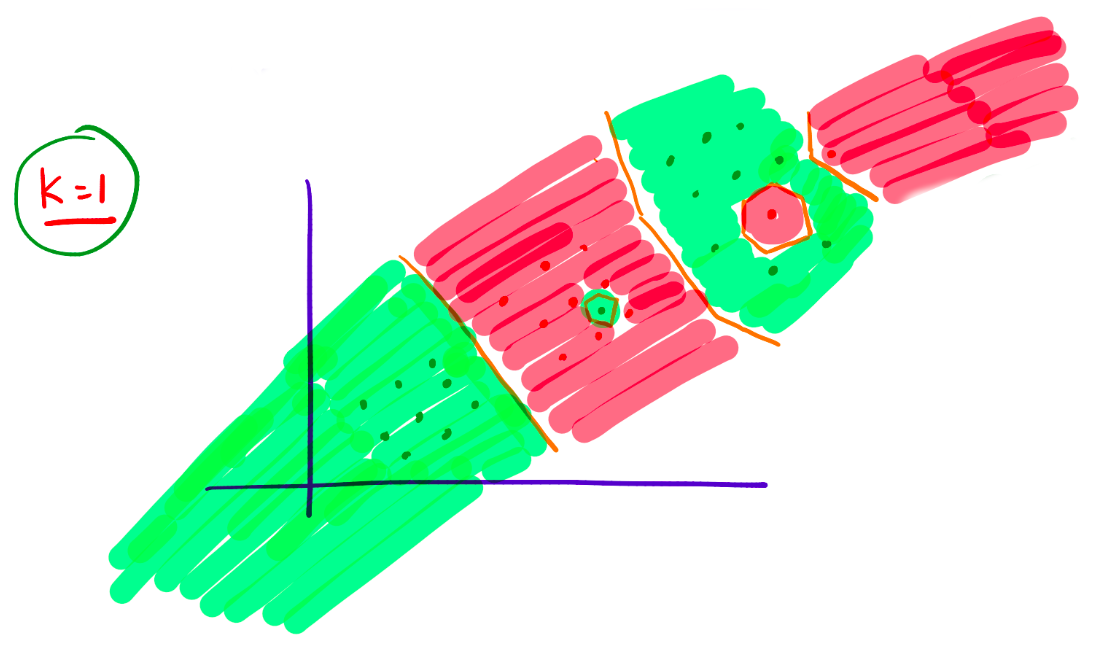
\includegraphics{../images/k1.png} \[
\text{When }k=1\text{, the classification is too sensitive to the outliers.}
\] 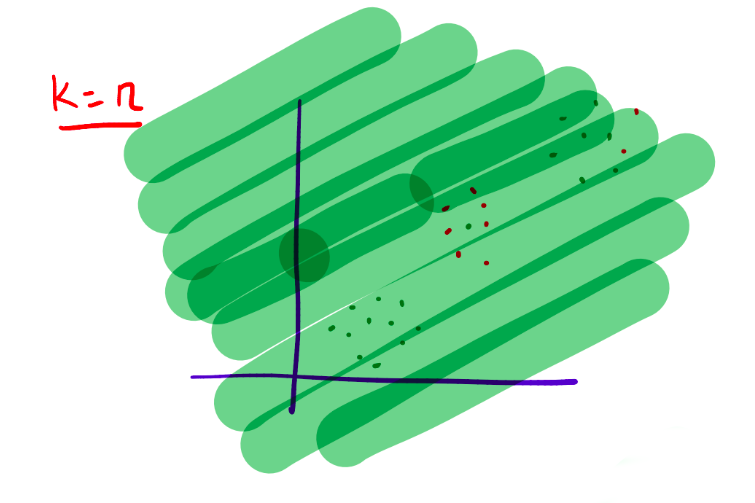
\includegraphics{../images/kn.png} \[
\text{When }k=n\text{, the classification is too smooth.}
\] 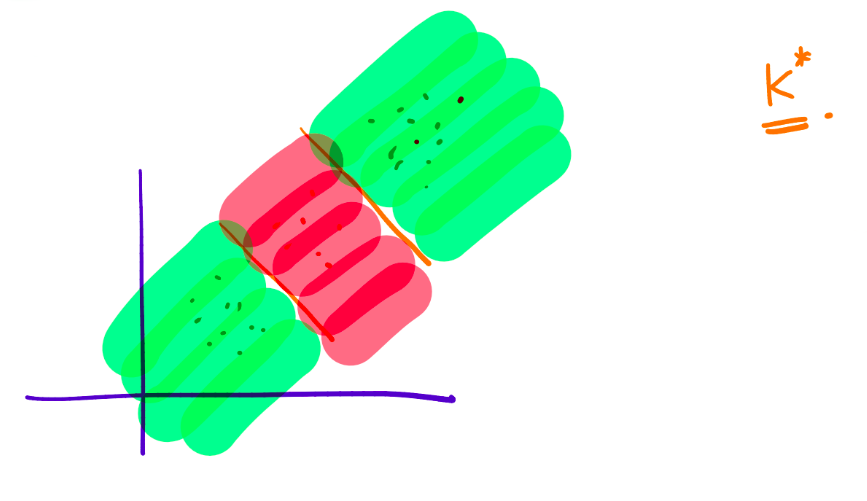
\includegraphics{../images/k*.png} \[
\text{When }k=k^*\text{, the classification is just right.}
\] The choice of \(k\) is usually done by cross-validation, where \(k\)
is treated as a hyper-parameter. The smaller \(k\) is, the more complex
the classification will be.

\newpage
\hypertarget{issues-with-k-nn}{%
\subsection{Issues with K-NN}\label{issues-with-k-nn}}

Following are the issues with the algorithm:

\begin{itemize}
\tightlist
\item
  The choice of distance function itself can give different results. The
  Euclidean distance might not always be the best fit!
\item
  It can be computationally demanding. When making a prediction for a
  single test datapoint, the distances between that datapoint and all
  training points must be calculated and sorted. As a result, the
  algorithm has a complexity of \(O(nlog(n))\), where \(n\) represents
  the size of the dataset.
\item
  No model is learned by this algorithm. It always needs the training
  dataset to make proper predictions.
\end{itemize}

\newpage
\hypertarget{introduction-to-decision-trees}{%
\section{Introduction to Decision
Trees}\label{introduction-to-decision-trees}}

Decision trees are a popular machine learning algorithm that operates by
recursively splitting the data based on the most informative features
until a stopping criterion is met. They are widely used for
classification and regression tasks and can be visualized as a tree-like
structure.

Given a dataset \(\{x_1, \ldots, x_n\}\) where \(x_i \in \mathbb{R}^d\),
let \(\{y_1, \ldots, y_n\}\) be the labels where \(y_i \in \{0, 1\}\).
The output of the algorithm will be a decision tree.

Prediction: Given \(x_{test}\), traverse through the tree to reach a
leaf node. \(y_{test} = \text{value in the leaf node}\).

Pictorial depiction of the decision tree:

\begin{figure}
\centering
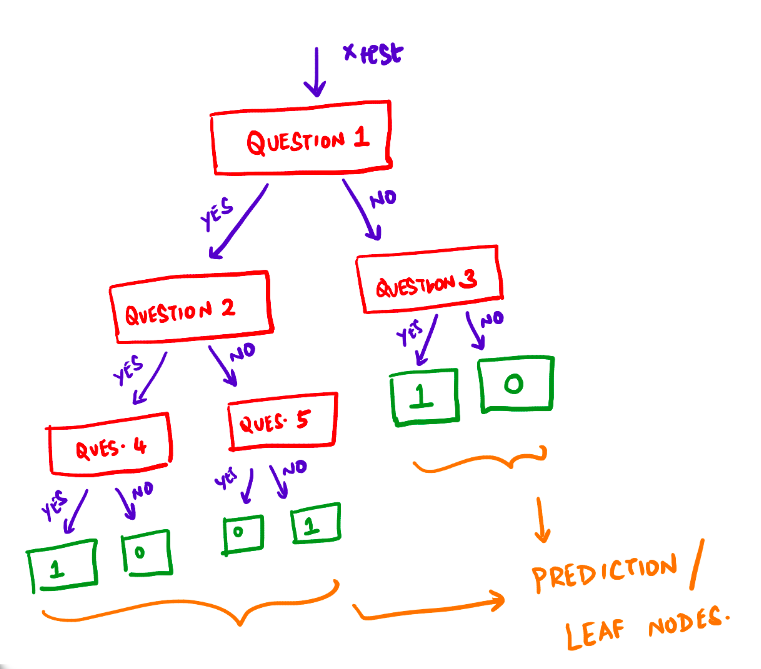
\includegraphics{../images/decision_tree.png}
\caption{Decision Tree}
\end{figure}

where a \textbf{question} is a (feature, value) pair. Example:
\(height\le180cm\)?

\hypertarget{goodness-of-a-question}{%
\subsection{Goodness of a Question}\label{goodness-of-a-question}}

Let \(D=\{(x_1, y_1), \ldots, (x_n,y_n)\}\) be the dataset. We partition
it using a question into \(D_{yes}\) and \(D_{no}\).

What we need is a measure of ``Impurity'' for a set of labels
\(\{y_1, \ldots, y_n\}\). This measure can be given by various ways, but
we will use the \textbf{Entropy} Function.

The Entropy function is given by, \[
Entropy(\{y_1, \ldots, y_n\}) = Entropy(p) = -\left( p\log(p)+(1-p)\log(1-p) \right )
\] where conventionally \(\log(0)\) is treated as \(0\).

Pictorial Representation of the Entropy function:

\begin{figure}
\centering
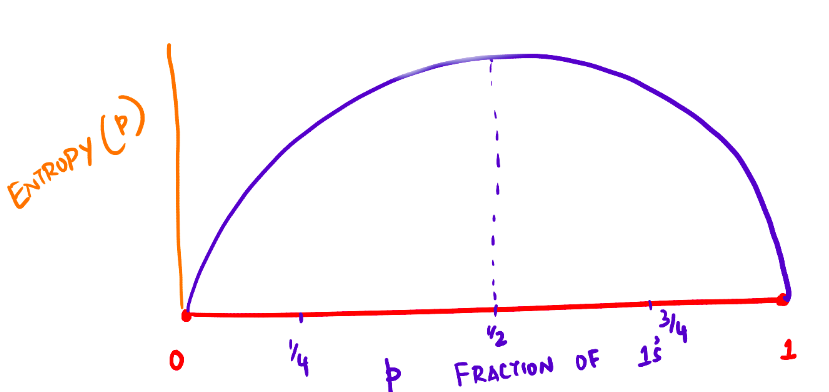
\includegraphics{../images/entropy.png}
\caption{Entropy Function}
\end{figure}

Then, we use Information Gain to measure the goodness of the split.

\textbf{Information gain} is a commonly used criterion in decision tree
algorithms that measures the reduction in entropy or impurity of a
dataset after splitting based on a given feature. By selecting features
with high information gain, decision trees can effectively differentiate
between the different classes of data and make accurate predictions.

Information gain is given by, \[
\text{Information Gain}(feature,value)=Entropy(D) - \left [ \gamma Entropy(D_{yes})+(1-\gamma)Entropy(D_{no}) \right ]
\] where \(\gamma\) is given by, \[
\gamma=\frac{|D_{yes}|}{|D|}
\]

\hypertarget{decision-tree-algorithm}{%
\subsection{Decision Tree Algorithm}\label{decision-tree-algorithm}}

The algorithm is as follows:

\begin{itemize}
\tightlist
\item
  Discretize each feature in {[}min,max{]} range.
\item
  Pick the question that has the largest information gain.
\item
  Repeat the procedure for \(D_{yes}\) and \(D_{no}\).
\item
  Stop growing the tree if a node becomes sufficiently ``pure''.
\end{itemize}

The goodness of a question can also be measured using different methods
like the Gini Index, etc.

Pictorial Depiction of decision boundary and its decision tree:

\begin{figure}
\centering
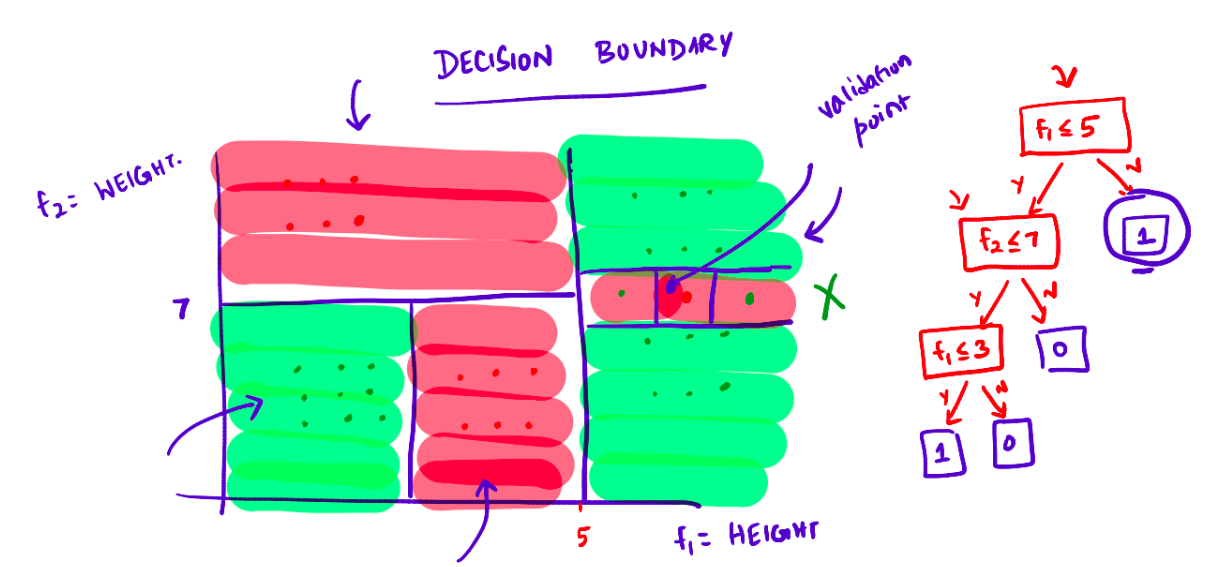
\includegraphics{../images/decision_bound.png}
\caption{Decision Boundary}
\end{figure}

\hypertarget{generative-and-discriminative-models}{%
\section{Generative and Discriminative
Models}\label{generative-and-discriminative-models}}

For the classical Classification problem, there are two types of
modeling: Generative and Discriminative Models.

Generative Models are given by, \[
P(x,y)
\] This primarily tries to model the feature generation.

Discriminative Models are given by, \[
P(y|x)
\] This only generates labels based on the data.

\hypertarget{credits}{%
\section{Credits}\label{credits}}

Professor Arun Rajkumar: The content as well as the notations are from
his slides and lecture.

\end{document}

\end{document}
